\documentclass[11pt]{article}
\usepackage[margin=1in]{geometry}
\usepackage{amsmath,amssymb}
\usepackage{graphicx}
\usepackage{booktabs}
\usepackage{xcolor}
\usepackage[hidelinks]{hyperref}

\graphicspath{{../nema_la_water_bgo/figures/}}

\newcommand{\code}[1]{\texttt{#1}}
\newcommand{\CRC}{\mathrm{CRC}}

\title{Reconstructing the Water NEMA IQ Phantom:\\
       Why Every Method Converges to the Same Frontier,\\
       and Where the Gap to Clinical Really Is}
\author{RecoCrysp --- MC reconstruction studies (Part III)}
\date{\today}

\begin{document}
\maketitle

\begin{abstract}
We reconstruct the full-physics water NEMA NU-2 image-quality phantom (six hot
spheres at 4:1 in a water cylinder, with attenuation, Compton scatter and randoms)
and compare a family of reconstruction methods against the clinical benchmark
(GE Discovery MI 3-ring, TOF-OSEM and Q.Clear; Vandendriessche et al.\ 2019). The
result is twofold and decisive. \emph{First}, every method that converges --- plain
MLEM with a post-filter, De~Pierro quadratic MAP-EM, one-step-late (OSL) edge priors,
and the convergent Q.Clear-style BSREM with the relative-difference prior (RDP) ---
collapses onto a \emph{single} contrast-recovery vs.\ background-variability frontier.
Edge-preserving priors buy nothing over a linear smoother here. \emph{Second}, and the
reason for the first: a reconstruction of the \emph{true} coincidences (gold; perfect
data, attenuation-corrected) already reproduces the clinical contrast-recovery curve to
within $\sim$1\%, whereas the \emph{corrected} reconstruction of the prompts sits
$\sim$24 contrast-recovery points below it. The entire deficit lives in the
scatter$+$randoms correction step, not in the reconstruction. The bottleneck is the
scatter (multiple-scatter) correction.
\end{abstract}

\section{Setup}
Phantom \code{nema\_la\_water\_bgo}: the NEMA NU-2 IQ phantom, six hot spheres
($\varnothing$ 10, 13, 17, 22, 28, 37\,mm) at a 4:1 hot:background ratio inside a water
body cylinder ($R=10$\,cm, half-length 9\,cm). All three physical corrections are
present and --- unlike the uniform sphere --- \emph{visible} in the metrics:
attenuation ($\mu_{\text{water}}=0.096\,\text{cm}^{-1}$ at 511\,keV), Compton scatter
(scatter fraction 20.5\%) and randoms (3.2\%). Data are PTCRYSP listmode coincidences,
classified by truth flag into trues / scatter / randoms.

We reconstruct three data sets per method:
\begin{itemize}
  \item \textbf{gold} --- true coincidences only, attenuation-corrected. The best case
        the pipeline can produce: perfect data, no contamination.
  \item \textbf{uncorr} --- all prompts (trues$+$scatter$+$randoms),
        attenuation-corrected, with \emph{no} scatter/randoms subtraction.
  \item \textbf{corr} --- all prompts, attenuation-corrected, minus our smoothed
        scatter$+$randoms contamination model.
\end{itemize}

\paragraph{Locked recipe.} $2.5$\,mm voxels ($91\times91\times73$); the
attenuation-weighted sensitivity $A^{\mathsf{T}}(a)$ sampled over $5\times10^{8}$ LORs
(below the Monte-Carlo noise floor) and cached once; 30 iterations (MLEM/MAP) or 60
(BSREM, whose relaxed steps converge more slowly).

\paragraph{Metric.} Per sphere we report the contrast recovery coefficient $\CRC$
(matching the NEMA contrast recovery, CR) and the NEMA \emph{background variability}
(BV; the standard deviation of size-matched background-ROI means over their mean), the
literature-standard noise metric. The clinical reference is the Discovery MI 3-ring
NEMA NU2-2012 IQ result (4:1).

\section{Methods attempted}
All share the same data, attenuation-weighted sensitivity and corrections; they differ
only in the image update.
\begin{itemize}
  \item \textbf{MLEM $+$ Gaussian post-filter} --- the linear-smoother baseline; the
        post-filter FWHM (0/4/6/8\,mm) trades contrast against noise.
  \item \textbf{De~Pierro quadratic MAP-EM} (\code{penalized\_mlem}) --- convergent,
        monotone; a quadratic smoothness prior.
  \item \textbf{OSL edge priors} (\code{osl\_mlem}) --- Huber, Logcosh and RDP via the
        one-step-late update. OSL is not a true surrogate: under attenuation (small
        central sensitivity) its denominator collapses and it diverges, so it carries a
        STIR-style denominator clamp and is usable only at low penalty strength
        ($\beta\!\lesssim\!10$).
  \item \textbf{BSREM $+$ RDP} (\code{bsrem}) --- the convergent, relaxed,
        preconditioned MAP algorithm behind GE Q.Clear, with the relative-difference
        prior. The prior enters the numerator (a true gradient term), not the EM
        denominator, so it is stable under attenuation with no clamp.
\end{itemize}

\section{Result 1: every method converges to the same linear frontier}
Figure~\ref{fig:frontier} shows the best operating point of each of the two
representative methods --- MLEM with no post-filter (\code{f0}, the highest-contrast
MLEM) and BSREM-RDP at its lowest stable penalty ($\beta=0.3$, the highest-contrast
BSREM). Both fall on the \emph{same} contrast-recovery curve (left) and the same point
on the contrast-vs-variability plane (right), well short of the clinical corner
(up-and-right). The full post-filter and $\beta$ sweeps (Table~\ref{tab:methods}), and
the De~Pierro quadratic and OSL Huber points, only slide each method \emph{along} this
one frontier --- never above it.

\begin{figure}[h]
  \centering
  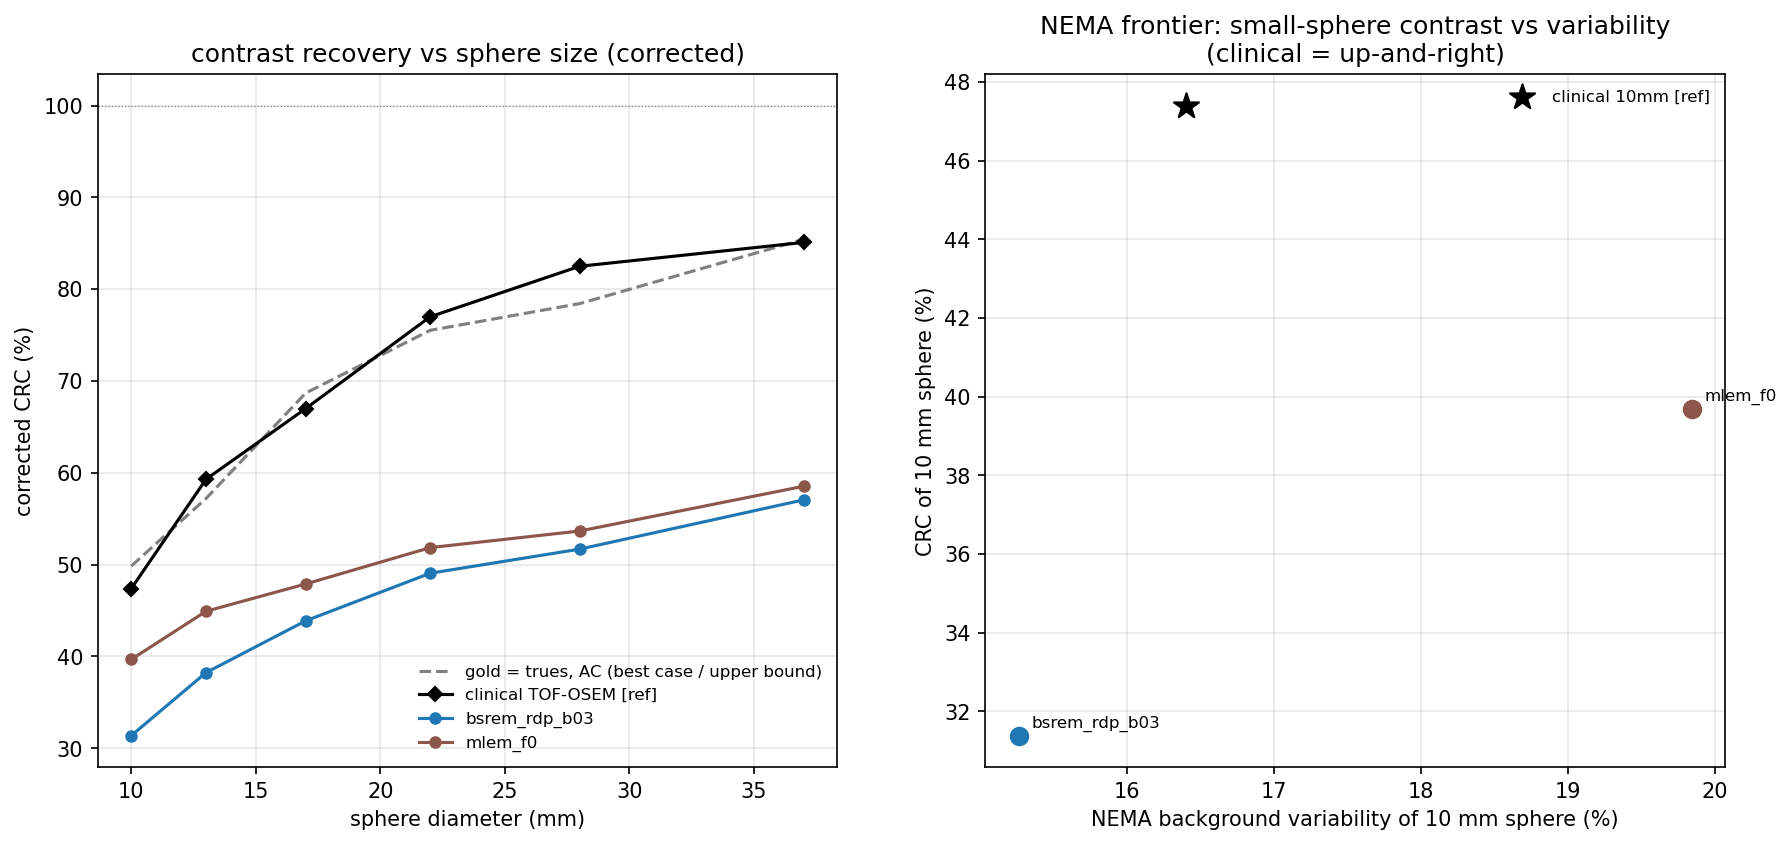
\includegraphics[width=\textwidth]{nema_la_water_bgo_compare_mlem_vs_bsrem.png}
  \caption{Best operating point of each method --- MLEM with no post-filter (\code{f0})
    and BSREM-RDP ($\beta=0.3$). Contrast recovery vs.\ sphere size (left) and the
    10\,mm contrast-recovery vs.\ background-variability point (right). Both land on the
    same curve, short of the clinical corner (up-and-right). ``Gold'' (grey dashed) is
    the trues-only upper bound, \emph{not} a target.}
  \label{fig:frontier}
\end{figure}

\begin{table}[h]
  \centering
  \caption{Reconstruction methods on the water NEMA phantom. 10\,mm-sphere operating
    points (corrected data). Every converging method sits on the same frontier;
    none reaches the clinical corner.}
  \label{tab:methods}
  \begin{tabular}{@{}llll@{}}
    \toprule
    Method & Algorithm class & Stable here? & 10\,mm $\CRC$/BV (\%) \\
    \midrule
    MLEM $+$ post-filter (f0/4/6/8) & linear smoother        & yes & 40/19.8 \dots\ 16/10.3 \\
    De~Pierro quadratic             & convergent, quadratic  & yes & 15/10.9 ($\beta$10) \\
    OSL Huber                       & one-step-late, edge    & $\beta\!\le\!10$ only & 30/14.4 ($\beta$3) \\
    OSL Logcosh / RDP               & one-step-late, edge    & OSL unstable under att. & --- \\
    \textbf{BSREM $+$ RDP} (Q.Clear)& convergent, edge       & yes (no clamp) & 31/15.3 \dots\ 27/12.9 \\
    \midrule
    Gold (trues, AC), any method    & ---                    & yes & $\approx$ clinical ($+1$) \\
    \bottomrule
  \end{tabular}
\end{table}

\section{Result 2: gold $=$ clinical; the gap is the corrections}
Why can no method beat the frontier? Because the frontier is set by the \emph{data}, not
the reconstruction. Figure~\ref{fig:decomp} shows the three reconstructions for one
representative method (BSREM-RDP, $\beta=0.5$): the gold curve (trues) rides the clinical
curve, while the corrected curve sits far below it, barely above the uncorrected one.

Table~\ref{tab:decomp} decomposes the loss (mean over the six spheres). The
reconstruction term is negligible ($\text{clinical}-\text{gold}=+1$\,pt). The
contamination removes $25$ contrast-recovery points if left in the data
($\text{gold}-\text{uncorr}$), and our correction model recovers only $1.6$ of them
($\text{corr}-\text{uncorr}$), leaving a $24$-point residual the model fails to recover
($\text{gold}-\text{corr}$). Randoms are only 3.2\% of prompts and cannot account for
this; the scatter pedestal (20.5\%) is the only term large enough, and it sits in the
corrected data essentially unsubtracted in and around the spheres.

\begin{figure}[h]
  \centering
  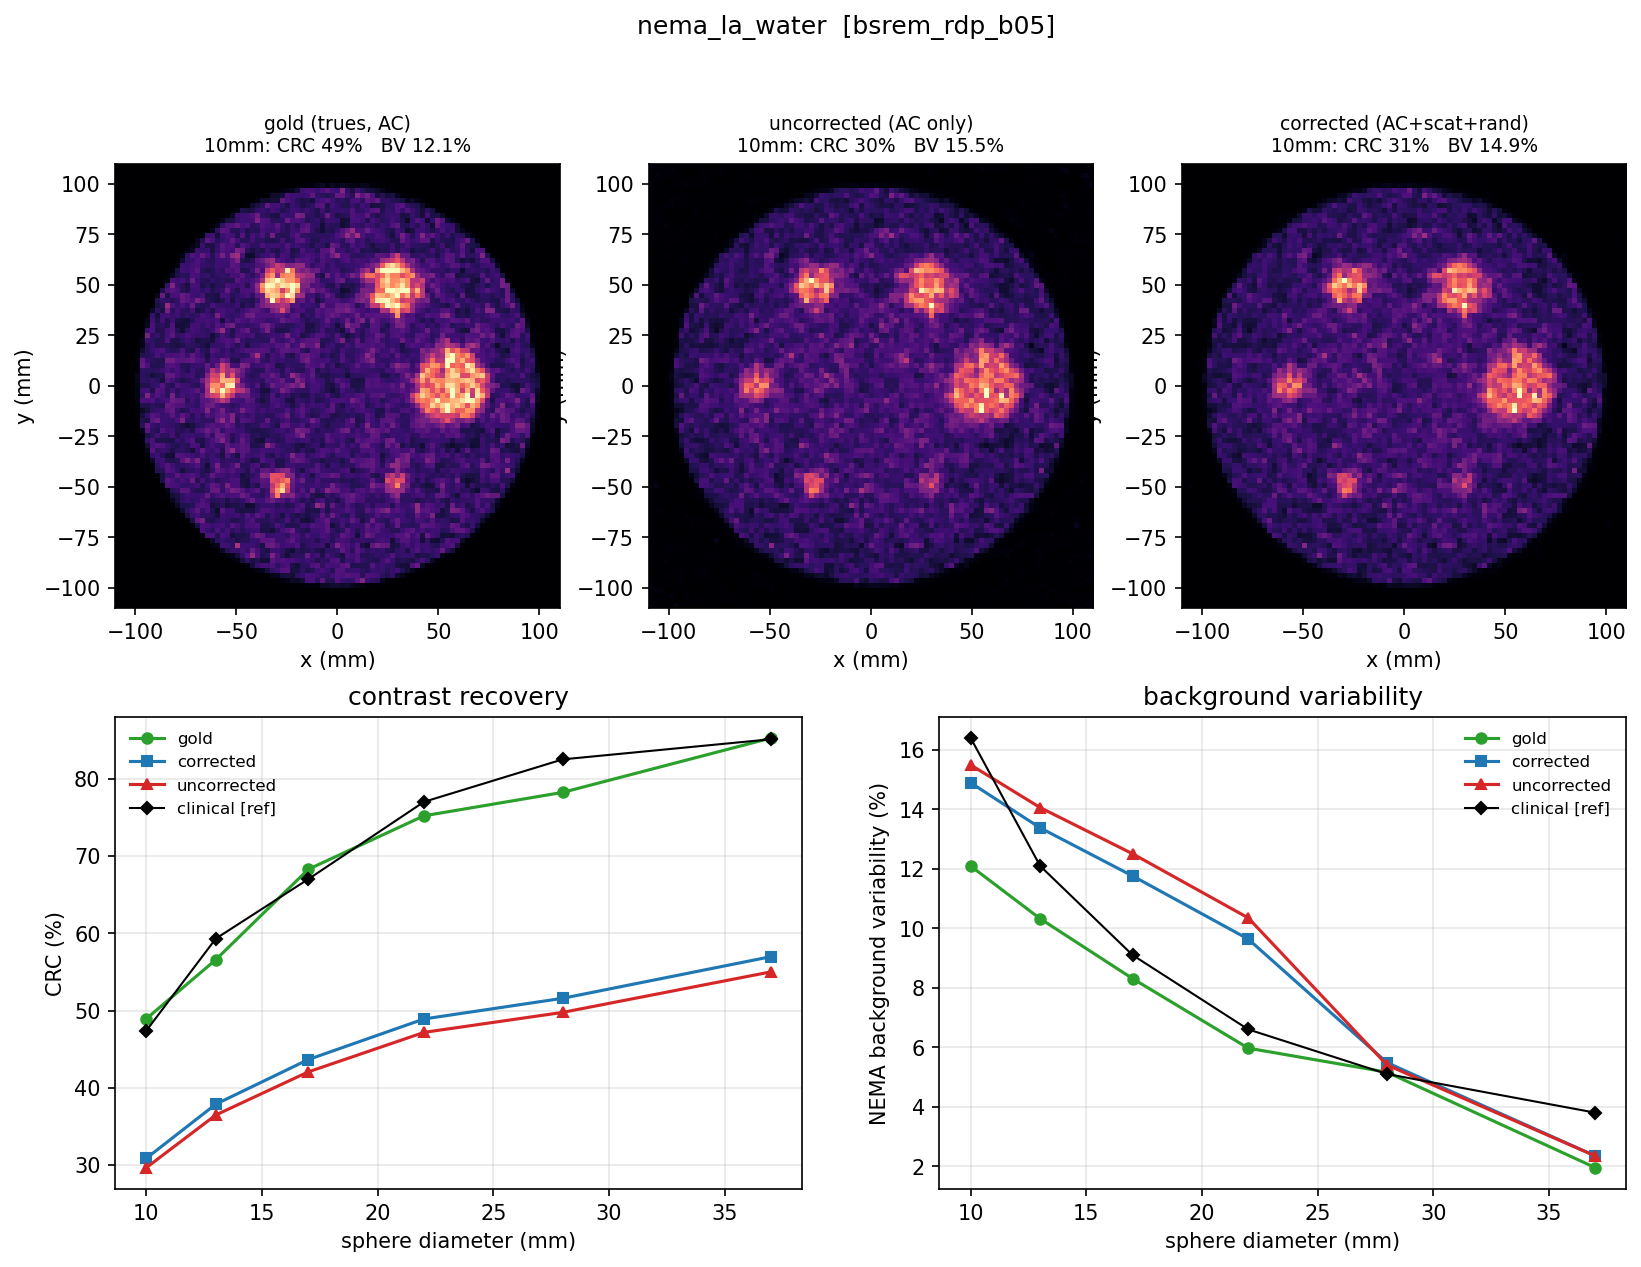
\includegraphics[width=\textwidth]{nema_la_water_bgo_bsrem_rdp_b05.png}
  \caption{Gold (trues, AC) / uncorrected (AC only) / corrected (AC$+$scatter$+$randoms)
    for BSREM-RDP ($\beta=0.5$). Top: central slices. Bottom: contrast recovery and NEMA
    background variability vs.\ sphere diameter, against the clinical reference. Gold
    tracks clinical; corrected falls $\sim$24 points below and barely improves on
    uncorrected --- the correction is almost a no-op where it matters.}
  \label{fig:decomp}
\end{figure}

\begin{table}[h]
  \centering
  \caption{Decomposition of the gold$\to$corrected contrast-recovery loss
    (mean over the six spheres, BSREM-RDP $\beta=0.5$; the MLEM points are
    within a point).}
  \label{tab:decomp}
  \begin{tabular}{@{}lll@{}}
    \toprule
    Step & Mean $\Delta\CRC$ & Meaning \\
    \midrule
    clinical $-$ gold   & $+1.0$  & reconstruction is fine (gold $=$ clinical) \\
    gold $-$ uncorr     & $+25.4$ & raw contamination damage \\
    corr $-$ uncorr     & $+1.6$  & recovered by our correction model \\
    gold $-$ corr       & $+23.8$ & residual the model fails to recover \\
    \bottomrule
  \end{tabular}
\end{table}

\section{Conclusion}
The reconstruction question is closed. With perfect data our reconstruction is already
clinical-grade (gold $=$ clinical to $\sim$1\%), and on the corrected data every
converging method --- linear smoother, quadratic MAP, OSL edge priors, convergent
BSREM-RDP --- collapses to the same contrast-vs-noise frontier. Edge-preserving priors
buy nothing here, because they all reconstruct the same contrast-suppressed corrected
data; no prior can recover contrast the correction step left out. Among the algorithms,
the convergent ones (De~Pierro, BSREM) are unconditionally stable under attenuation,
while OSL needs a denominator clamp and still breaks above $\beta\!\approx\!10$; BSREM is
therefore the right default for edge priors --- but the point is moot until the data are
better corrected.

The lever is the \textbf{scatter (multiple-scatter) correction}: it recovers $1.6$ of
the $25$ contrast-recovery points scatter removes. Fixing it is worth $\sim$24 points and
is the only route left to the clinical curve. Re-scanning reconstruction priors is not.

\end{document}
